\section{Why MLOps?}

% --- SLIDE 1: THE FRAMING ---
\begin{frame}{Everything So Far Ended at \texttt{model.fit()}}

    \centering
    \large
    \textit{Every deck in this course stops at the same place: a trained model, in a notebook, on your laptop.}

    \vspace{0.36em}

    \begin{columns}[T]
        \begin{column}{0.46\textwidth}
            \begin{tcolorbox}[colback=blue!5, colframe=blue!50, title=What we have taught you]
                \scriptsize
                \begin{itemize}
                    \item Split the data, pick a metric
                    \item Fit a model, tune it a bit
                    \item Report a validation score
                \end{itemize}
            \end{tcolorbox}
        \end{column}
        \begin{column}{0.46\textwidth}
            \begin{tcolorbox}[colback=red!5, colframe=red!50, title=What nobody taught you]
                \scriptsize
                \begin{itemize}
                    \item Which run produced that number?
                    \item Can you rebuild it in six months?
                    \item Who calls the model, and what happens when it is wrong?
                    \item How will you know it stopped working?
                \end{itemize}
            \end{tcolorbox}
        \end{column}
    \end{columns}

    \vspace{0.3em}
    \scriptsize
    \textbf{MLOps} is the set of practices that answers the right-hand column.

\end{frame}

% --- SLIDE 2: SCULLEY'S SMALL BOX ---
\begin{frame}{The ML Code Is the Small Box}

    \centering
    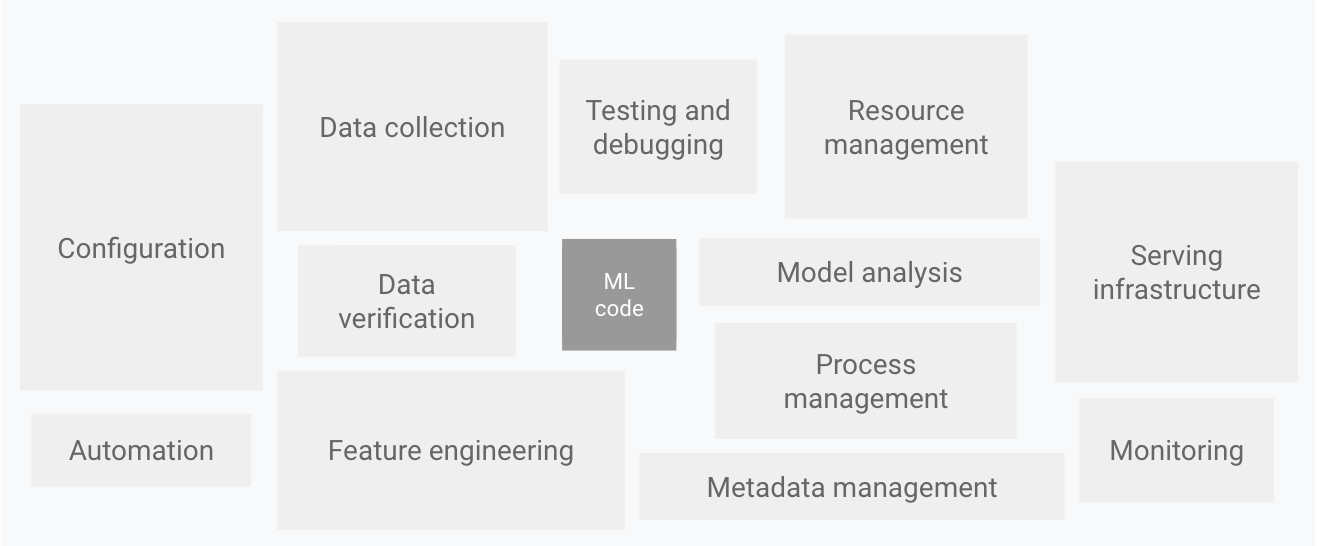
\includegraphics[width=0.92\textwidth,height=0.42\textheight,keepaspectratio]{images/mlops-foundations/gcp_elements_of_ml.png}

    {\scriptsize Source: Google Cloud, ``MLOps: Continuous delivery and automation pipelines in machine learning,''
    \href{https://cloud.google.com/architecture/mlops-continuous-delivery-and-automation-pipelines-in-machine-learning}{Cloud Architecture Center},
    Figure~1 --- after Sculley et al., \textit{Hidden Technical Debt in Machine Learning Systems}, NeurIPS 2015, Figure~1.}

    \vspace{0.6em}
    \begin{itemize}
        \item Sculley et al.\ (2015): ``\textit{Only a small fraction of real-world ML systems is composed of the ML code
              \ldots\ the required surrounding infrastructure is vast and complex.}''
        \item The grey box is what this course has been about. Everything around it is what makes it \emph{useful}.
    \end{itemize}

\end{frame}

% --- SLIDE 3: HIDDEN TECHNICAL DEBT ---
\begin{frame}{Hidden Technical Debt}

    \begin{block}{The core argument (Sculley et al., NeurIPS 2015)}
        Building an ML system is fast and cheap. \textbf{Maintaining} it is slow and expensive.
        The debt is \emph{hidden} because it lives at the system level, not in the code, so ordinary
        code review and unit tests do not find it.
    \end{block}

    \vspace{0.5em}
    \begin{columns}[T]
        \begin{column}{0.48\textwidth}
            \small
            \textbf{Boundary erosion}
            \begin{itemize}
                \item \textbf{Entanglement (CACE):} \textit{Changing Anything Changes Everything}. Change one
                      feature's distribution and every other weight shifts.
                \item \textbf{Correction cascades:} a model that patches another model's output --- now you cannot
                      improve either one alone.
                \item \textbf{Undeclared consumers:} someone reads your predictions off a log and you never find out.
            \end{itemize}
        \end{column}
        \begin{column}{0.48\textwidth}
            \small
            \textbf{System-level anti-patterns}
            \begin{itemize}
                \item \textbf{Glue code:} 95\% of the repository is plumbing around a 5\% library call.
                \item \textbf{Pipeline jungles:} scrapes and joins accreted over years; nobody can rerun them.
                \item \textbf{Configuration debt:} a hundred flags, no schema, no review.
                \item \textbf{Feedback loops:} the model influences the data it will next be trained on.
            \end{itemize}
        \end{column}
    \end{columns}

\end{frame}

% --- SLIDE 4: WHAT ACTUALLY BREAKS ---
\begin{frame}{What Actually Breaks After Deployment}

    \centering
    \textit{None of these are modelling problems. All of them are engineering problems.}
    \vspace{0.18em}

    \renewcommand{\arraystretch}{1.35}
    {\scriptsize
    \begin{tabular}{p{4.0cm}|p{7.4cm}}
        \toprule
        \textbf{Symptom} & \textbf{Actual cause} \\
        \midrule
        Accuracy fell off a cliff overnight & An upstream team renamed a column; your feature is now all-null \\
        Accuracy decayed slowly over a year & The world changed; your training distribution did not \\
        ``Works on my machine'' & Unpinned dependency; a minor version bumped a default \\
        Cannot reproduce last quarter's model & The training data was overwritten in place \\
        Two teams report different numbers & Different splits, different seeds, different preprocessing \\
        Nobody noticed for three months & Nothing was monitored except server uptime \\
        \bottomrule
    \end{tabular}}

    \vspace{0.24em}
    {\scriptsize See Paleyes, Urma \& Lawrence, ``Challenges in Deploying Machine Learning: a Survey of Case Studies,''
    \textit{ACM Computing Surveys}, 2022, \href{https://arxiv.org/abs/2011.09926v3}{arXiv:2011.09926v3}, for a
    catalogue of these from published industry post-mortems.}

\end{frame}

% --- SLIDE 5: WHAT IS MLOPS ---
\begin{frame}{So What Is MLOps?}

    \begin{block}{Working definition}
        \textbf{MLOps} applies DevOps practices --- version control, automated testing, continuous integration and
        delivery, monitoring --- to machine learning systems, where the deliverable is not just code but
        \textbf{code + data + model} together.
    \end{block}

    \vspace{0.5em}
    \centering
    \begin{tikzpicture}[
        node distance=0.6cm,
        box/.style={rectangle, draw, rounded corners=2pt, minimum height=1.0cm, text width=2.6cm,
                    align=center, font=\small},
        lbl/.style={font=\scriptsize\itshape, text=gray!70!black}
    ]
        \node[box, fill=blue!10]  (code)  {\textbf{Code}};
        \node[box, fill=green!10, right=of code]  (data)  {\textbf{Data}};
        \node[box, fill=orange!10, right=of data] (model) {\textbf{Model}};
        \node[box, fill=gray!12, right=of model]  (cfg)   {\textbf{Config}};

        \node[lbl, below=1mm of code]  {git, reviewed};
        \node[lbl, below=1mm of data]  {versioned, hashed};
        \node[lbl, below=1mm of model] {registered, staged};
        \node[lbl, below=1mm of cfg]   {declared, validated};

        \node[font=\small, above=3mm of data, xshift=1.7cm]
            {A deployment is a \emph{tuple} of all four --- not a single commit.};
    \end{tikzpicture}

    \vspace{1.2em}
    \begin{itemize}
        \item \textbf{Not} a product you buy. \textbf{Not} a job title you hire once. It is a set of habits plus
              a small amount of tooling.
        \item The habits matter more than the tools. A team with a spreadsheet and discipline beats a team with
              a platform and none.
    \end{itemize}

\end{frame}
